\subsection{Μελέτη επίδρασης παραμέτρων ιεραρχίας μνήμης στην απόδοση της εφαρμογής θεωρώντας σταθερό κύκλο ρολογιού}
\vspace{3mm}

%----------------L1 Cache-----------------------
\subsubsection{L1 Cache}
Οι παράμετροι της \textlatin{L2 cache} και του \textlatin{TLB} θα διατηρηθούν
σταθερές και συγκεκριμένα ίσες με:


\begin{multicols}{2}
    \begin{itemize}
        \item L2 size = 1024 KB  
        \item L2 associativity = 8
        \item L2 block size = 128 B
        \item TLB size = 64 entr.
        \item TLB associativity = 4
        \item TLB page size = 4096 B
    \end{itemize}
\end{multicols}

Ακολουθούν τα διαγράμματα που προέκυψαν και ο σχετικός σχολιασμός τους:

\begin{minipage}{\textwidth}
    \begin{center}
        \fbox{\textlatin{\textbf{\textit{blackscholes}}}}\\
        \vspace{3mm}
        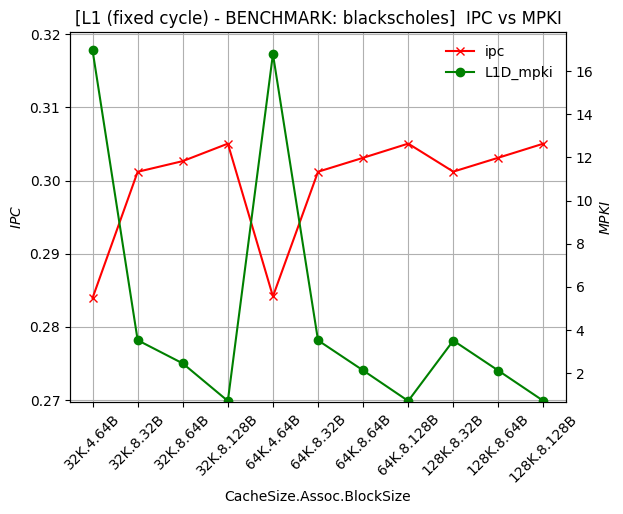
\includegraphics[scale=0.70]{graphs/L1/fixed/blackscholes.png}
        \vspace{6mm}
    \end{center}
\end{minipage}


\begin{minipage}{\textwidth}
    \begin{center}
        \fbox{\textlatin{\textbf{\textit{bodytrack}}}}\\
        \vspace{3mm}
        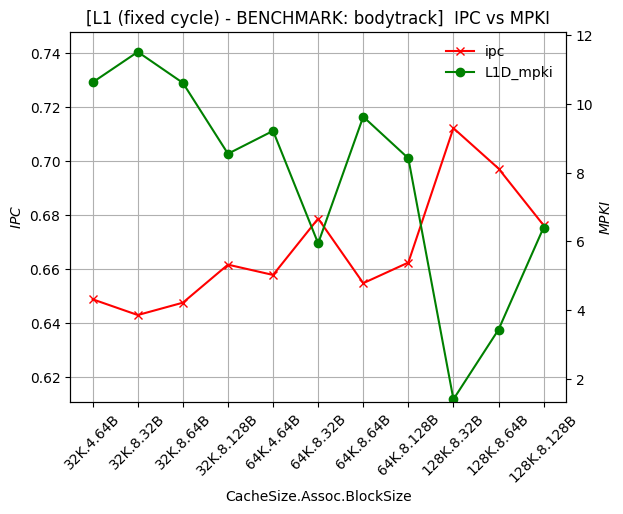
\includegraphics[scale=0.70]{graphs/L1/fixed/bodytrack.png}
        \vspace{6mm}
    \end{center}
\end{minipage}

\begin{minipage}{\textwidth}
    \begin{center}
        \fbox{\textlatin{\textbf{\textit{canneal}}}}\\
        \vspace{3mm}
        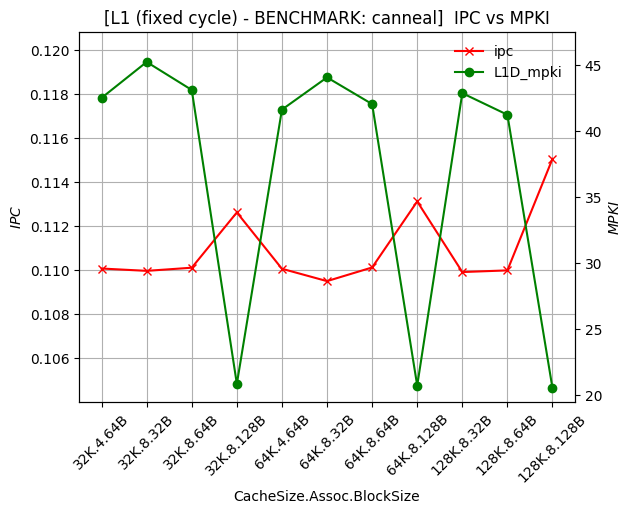
\includegraphics[scale=0.70]{graphs/L1/fixed/canneal.png}
        \vspace{6mm}
    \end{center}
\end{minipage}

\begin{minipage}{\textwidth}
    \begin{center}
        \fbox{\textlatin{\textbf{\textit{facesim}}}}\\
        \vspace{3mm}
        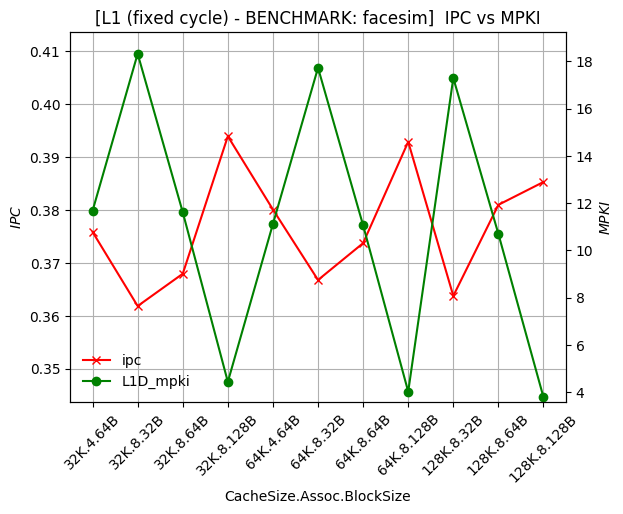
\includegraphics[scale=0.70]{graphs/L1/fixed/facesim.png}
        \vspace{6mm}
    \end{center}
\end{minipage}

\begin{minipage}{\textwidth}
    \begin{center}
        \fbox{\textlatin{\textbf{\textit{ferret}}}}\\
        \vspace{3mm}
        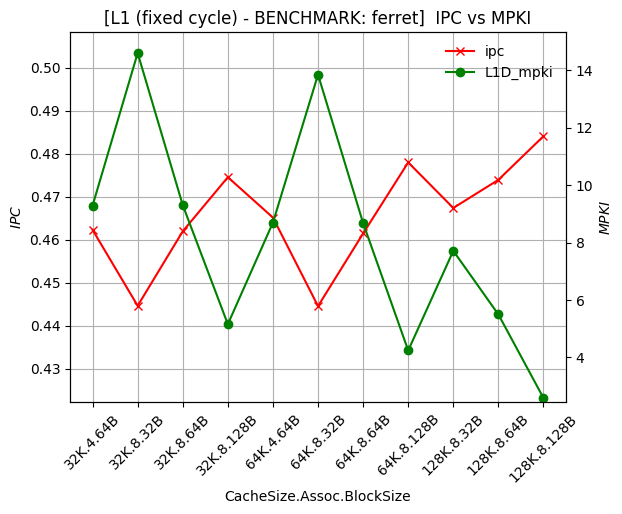
\includegraphics[scale=0.70]{graphs/L1/fixed/ferret.png}
        \vspace{6mm}
    \end{center}
\end{minipage}


\begin{minipage}{\textwidth}
    \begin{center}
        \fbox{\textlatin{\textbf{\textit{fluidanimate}}}}\\
        \vspace{3mm}
        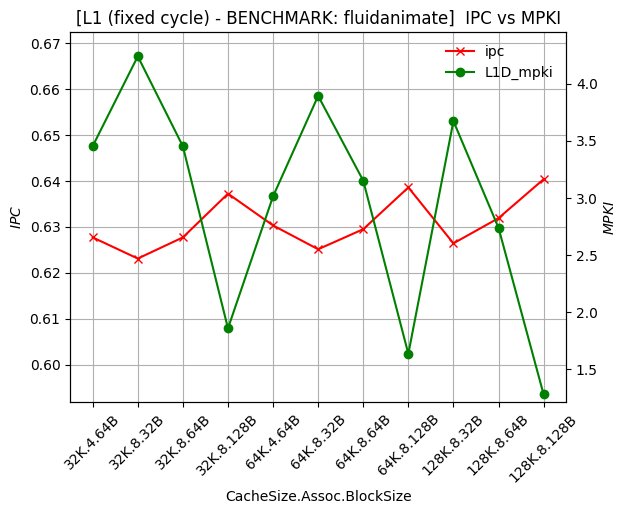
\includegraphics[scale=0.70]{graphs/L1/fixed/fluidanimate.png}
        \vspace{6mm}
    \end{center}
\end{minipage}

\begin{minipage}{\textwidth}
    \begin{center}
        \fbox{\textlatin{\textbf{\textit{freqmine}}}}\\
        \vspace{3mm}
        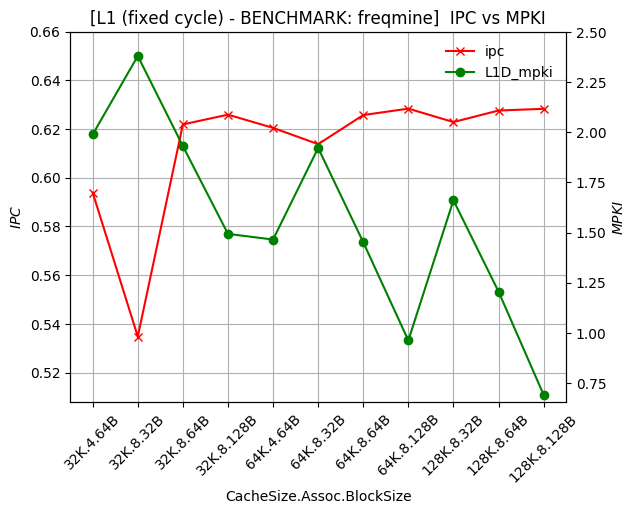
\includegraphics[scale=0.70]{graphs/L1/fixed/freqmine.png}
        \vspace{6mm}
    \end{center}
\end{minipage}

\begin{minipage}{\textwidth}
    \begin{center}
        \fbox{\textlatin{\textbf{\textit{rtview}}}}\\
        \vspace{3mm}
        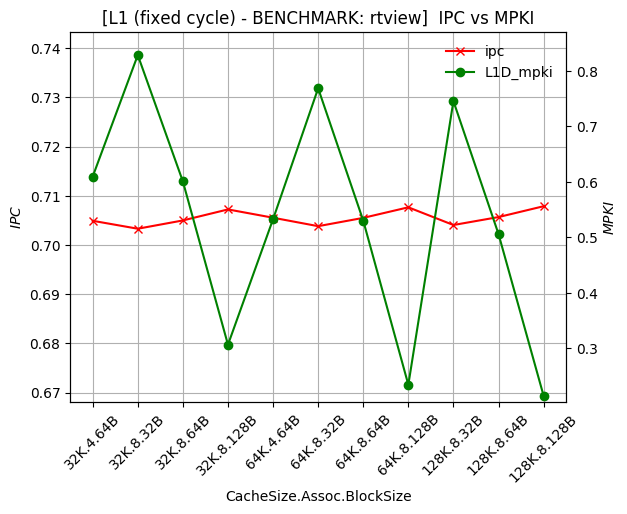
\includegraphics[scale=0.70]{graphs/L1/fixed/rtview.png}
        \vspace{6mm}
    \end{center}
\end{minipage}

\begin{minipage}{\textwidth}
    \begin{center}
        \fbox{\textlatin{\textbf{\textit{streamcluster}}}}\\
        \vspace{3mm}
        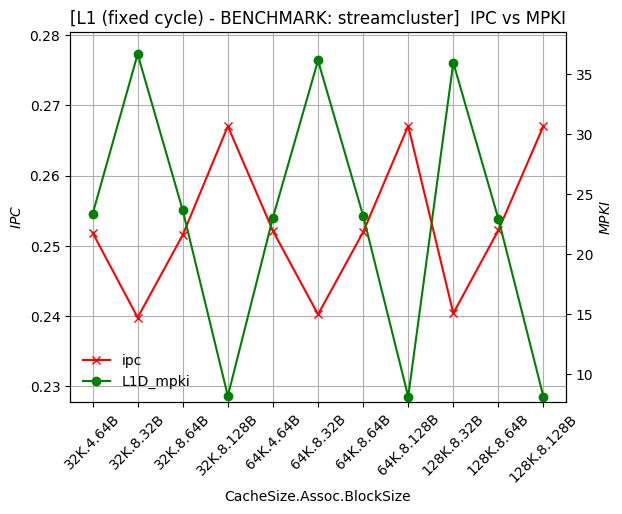
\includegraphics[scale=0.70]{graphs/L1/fixed/streamcluster.png}
        \vspace{6mm}
    \end{center}
\end{minipage}

\begin{minipage}{\textwidth}
    \begin{center}
        \fbox{\textlatin{\textbf{\textit{swaptions}}}}\\
        \vspace{3mm}
        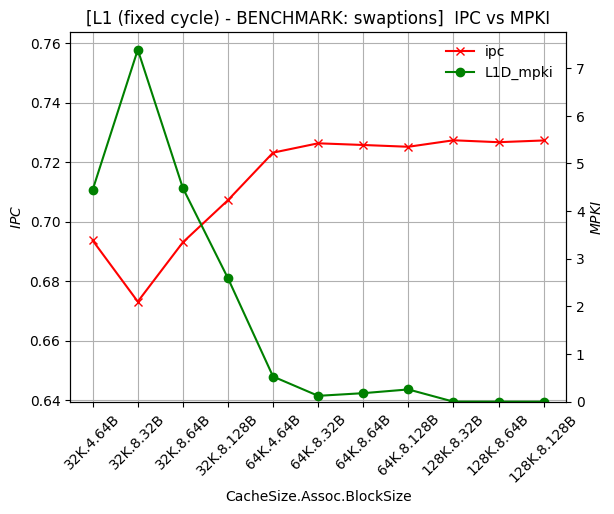
\includegraphics[scale=0.70]{graphs/L1/fixed/swaptions.png}
        \vspace{6mm}
    \end{center}
\end{minipage}

Επίσης, για λόγους συνολικής εποπτείας παρατίθεται ένα διάγραμμα των γεωμετρικών μέσων των προηγούμενων:\\\\
\begin{minipage}{\textwidth}
    \begin{center}
        \fbox{\textlatin{\textbf{\textit{Geometric Average}}}}\\
        \vspace{3mm}
        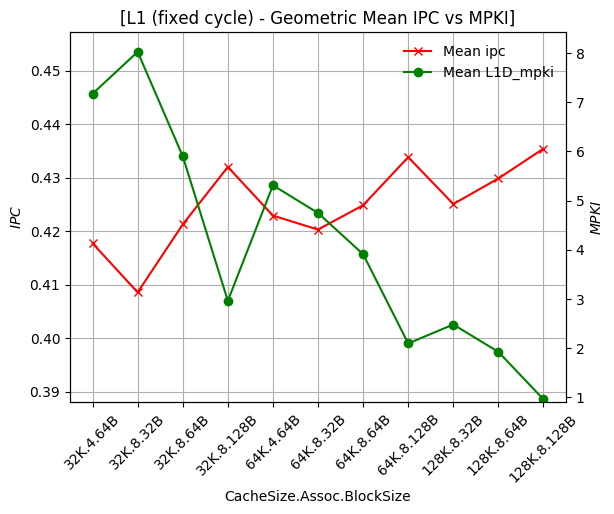
\includegraphics[scale=0.60]{graphs/L1/fixed/mean.png}
        \vspace{6mm}
    \end{center}
\end{minipage}




\begin{center}
    \textbf{Συμπεράσματα για την \textlatin{L1 Cache}}    
\end{center}

Παρατηρούμε πως τα μεγέθη Instructions Per Cycle και Misses Per KiloInstructions
μεταβάλλονται αντιστρόφως ανάλογα. Αυτό σαφώς είναι αναμενόμενο, αφού όσο
περισσότερες αστοχίες υπάρχουν (μεγαλύτερο MPKI), τόσο περισσότεροι κύκλοι
χρειάζονται για να εκτελεστεί η εντολή και άρα η επίδοση θα είναι χειρότερη,
δηλαδή το IPC θα είναι μικρότερο, και αντίστροφα. 

\begin{enumerate}
    \item Παρατηρούμε πως σχεδόν σε όλα τα \textlatin{benchmarks} με εξαίρεση το
    \textlatin{swaptions}, η μεταβολή του μεγέθους της \textlatin{cache} δεν
    επηρεάζει αρκετά το \textlatin{IPC}. Αυτό θα μπορούσε να ερμηνευθεί από το
    ότι ενδεχομένως στα \textlatin{benchmarks} αυτά, τα \textlatin{misses}
    οφείλονται κυρίως σε \textlatin{compulsory misses} και όχι
    σε \textlatin{capacity misses}.
    
    \item Στο \textlatin{benchmark blackscholes}, παρατηρούμε πως η αύξηση του
    \textlatin{associativity} αύξησε το \textlatin{IPC} και μείωσε το
    \textlatin{MPKI} (μειώθηκαν τα \textlatin{conflict misses}).
    
    \item Στα \textlatin{benchmarks bodytrack, canneal, facesim, ferret,
    fluidanimate, streamcluster, swaptions} (σε άλλα περισσότερο και σε άλλα
    λιγότερο, σε άλλα κυρίως για μικρότερες τιμές μεγέθους της
    \textlatin{cache}), παρατηρούμε ότι η αύξηση του \textlatin{block size}
    οδηγεί στην αύξηση του \textlatin{IPC} και επομένως στη μείωση των
    \textlatin{MPKI} ( \textlatin{compulsory misses} κατά κύριο λόγο).
    
    \item Το \textlatin{benchmark rtview} είναι εκείνο που επηρεάζεται λιγότερο
    από τις αλλαγές των παραμέτρων. Συγκεκριμένα το \textlatin{IPC} κυμαίνεται
    μεταξύ $0.70-0.71$, ενώ ταυτόχρονα τα \textlatin{MPKI} μεταξύ $0.2-0.75$
    περίπου. 

    \item Το bencmark swaptions φαίνεται να επηρεάζεται καθοριστικά από το
    μέγεθος της L1 Cache. Η επιλογή L1 Cache Size μεγαλύτερο ή ίσο των 64Κ
    βελτιώνει δραματικά την επίδοση.
\end{enumerate}

Σαν γενικό συμπέρασμα, βλέπουμε ότι το \textlatin{block size} και το associativity επηρεάζουν σε
βαθμό σε σχέση με τo Cache Size.
\vspace{1cm}

\textit{Θα μπορούσαμε να πούμε με βάση τις παραπάνω μετρήσεις, ότι οι συνδυασμοί 64Κ.8.128Β και 128Κ.8.128B αποτελούν τις καλύτερες επιλογές μας αναφορικά με την \textlatin{L1 Cache}.}

%\newpage ----------------L2 Cache-----------------------
\newpage
\subsubsection{L2 Cache}
Οι παράμετροι της \textlatin{L1 cache} και του \textlatin{TLB} θα διατηρηθούν
σταθερές και συγκεκριμένα ίσες με:

\begin{multicols}{2}
    \begin{itemize}
        \item L1 size = 32 KB  
        \item L1 associativity = 8
        \item L1 block size = 64 B
        \item TLB size = 64 entr.
        \item TLB associativity = 4
        \item TLB page size = 4096 B
    \end{itemize}
\end{multicols}

\begin{minipage}{\textwidth}
    \begin{center}
        \fbox{\textlatin{\textbf{\textit{blackscholes}}}}\\
        \vspace{3mm}
        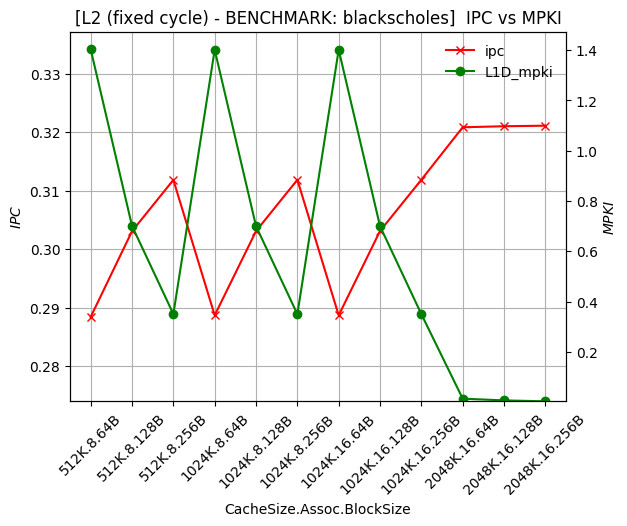
\includegraphics[scale=0.70]{graphs/L2/fixed/blackscholes.png}
        \vspace{6mm}
    \end{center}
\end{minipage}


\begin{minipage}{\textwidth}
    \begin{center}
        \fbox{\textlatin{\textbf{\textit{bodytrack}}}}\\
        \vspace{3mm}
        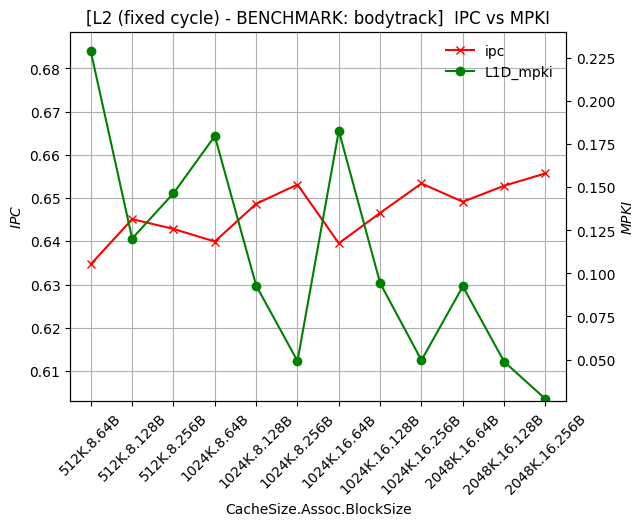
\includegraphics[scale=0.70]{graphs/L2/fixed/bodytrack.png}
        \vspace{6mm}
    \end{center}
\end{minipage}

\begin{minipage}{\textwidth}
    \begin{center}
        \fbox{\textlatin{\textbf{\textit{canneal}}}}\\
        \vspace{3mm}
        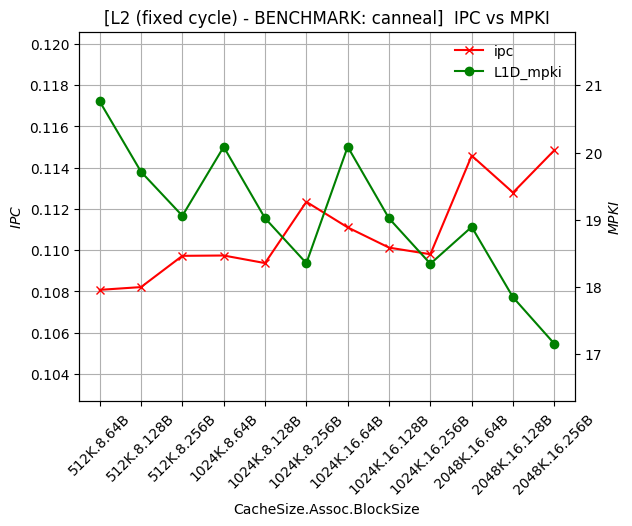
\includegraphics[scale=0.70]{graphs/L2/fixed/canneal.png}
        \vspace{6mm}
    \end{center}
\end{minipage}

\begin{minipage}{\textwidth}
    \begin{center}
        \fbox{\textlatin{\textbf{\textit{facesim}}}}\\
        \vspace{3mm}
        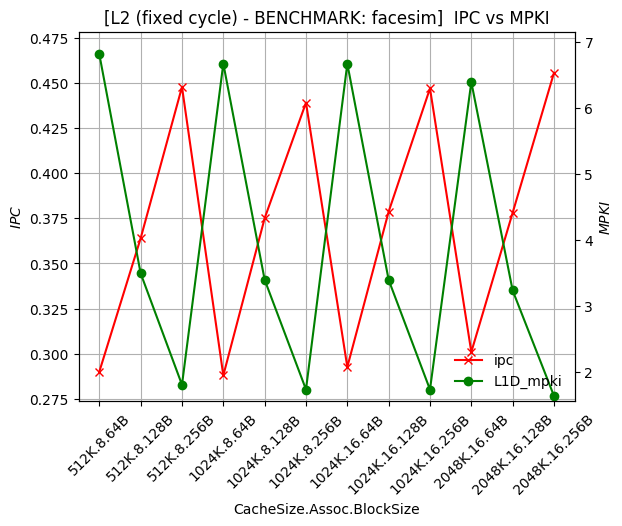
\includegraphics[scale=0.70]{graphs/L2/fixed/facesim.png}
        \vspace{6mm}
    \end{center}
\end{minipage}

\begin{minipage}{\textwidth}
    \begin{center}
        \fbox{\textlatin{\textbf{\textit{ferret}}}}\\
        \vspace{3mm}
        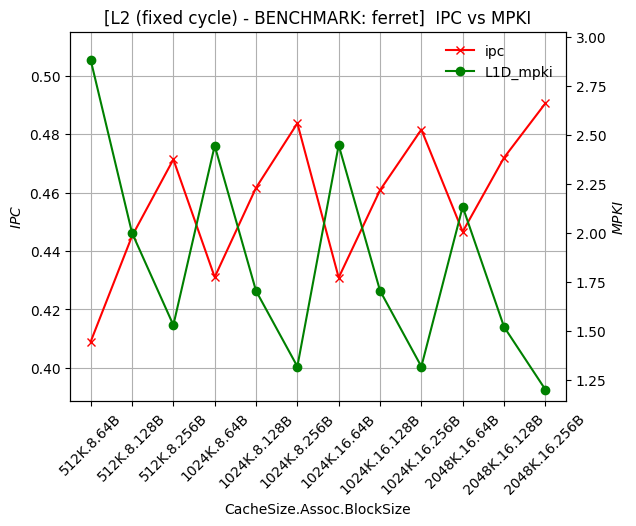
\includegraphics[scale=0.70]{graphs/L2/fixed/ferret.png}
        \vspace{6mm}
    \end{center}
\end{minipage}


\begin{minipage}{\textwidth}
    \begin{center}
        \fbox{\textlatin{\textbf{\textit{fluidanimate}}}}\\
        \vspace{3mm}
        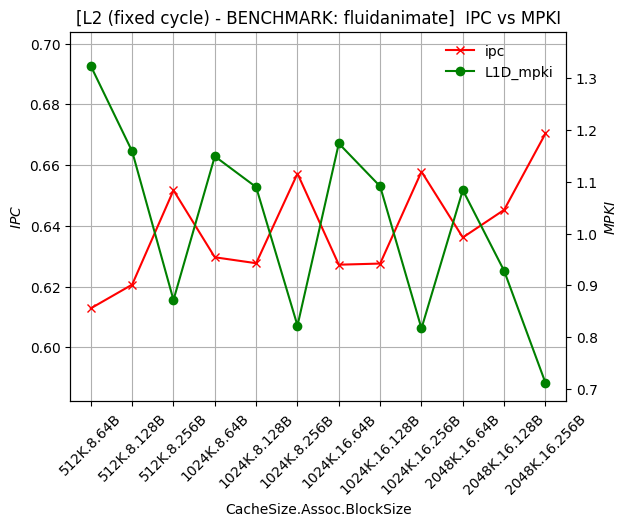
\includegraphics[scale=0.70]{graphs/L2/fixed/fluidanimate.png}
        \vspace{6mm}
    \end{center}
\end{minipage}

\begin{minipage}{\textwidth}
    \begin{center}
        \fbox{\textlatin{\textbf{\textit{freqmine}}}}\\
        \vspace{3mm}
        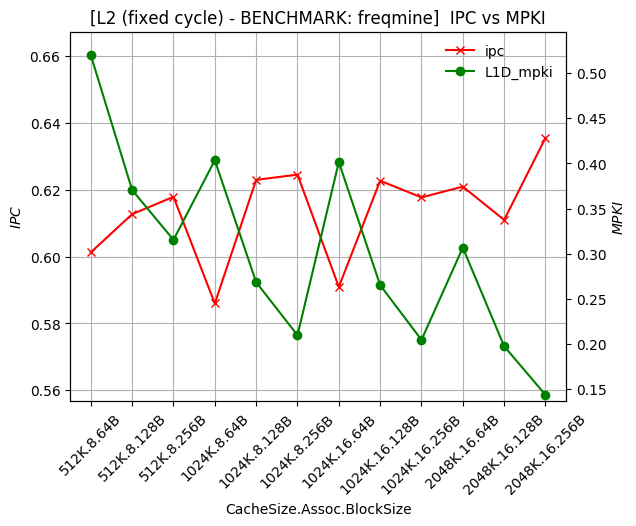
\includegraphics[scale=0.70]{graphs/L2/fixed/freqmine.png}
        \vspace{6mm}
    \end{center}
\end{minipage}

\begin{minipage}{\textwidth}
    \begin{center}
        \fbox{\textlatin{\textbf{\textit{rtview}}}}\\
        \vspace{3mm}
        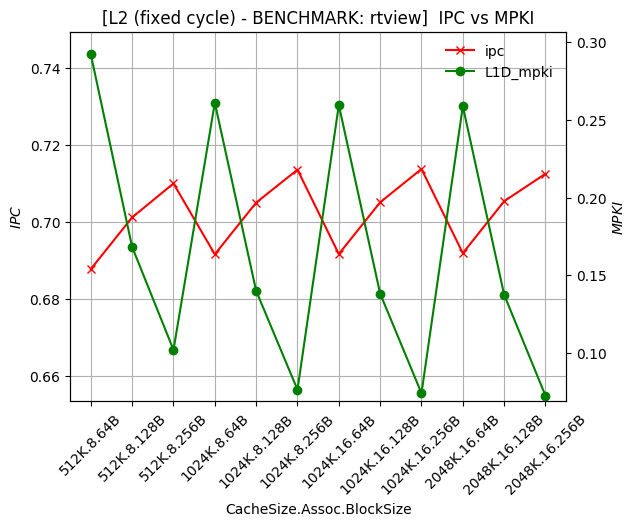
\includegraphics[scale=0.70]{graphs/L2/fixed/rtview.png}
        \vspace{6mm}
    \end{center}
\end{minipage}

\begin{minipage}{\textwidth}
    \begin{center}
        \fbox{\textlatin{\textbf{\textit{streamcluster}}}}\\
        \vspace{3mm}
        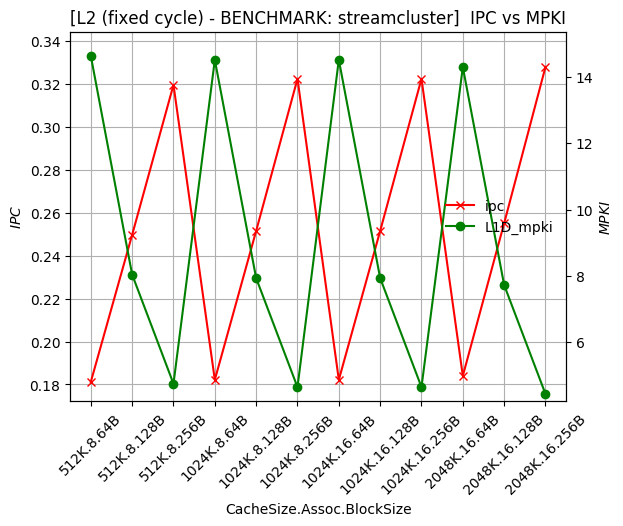
\includegraphics[scale=0.70]{graphs/L2/fixed/streamcluster.png}
        \vspace{6mm}
    \end{center}
\end{minipage}

\begin{minipage}{\textwidth}
    \begin{center}
        \fbox{\textlatin{\textbf{\textit{swaptions}}}}\\
        \vspace{3mm}
        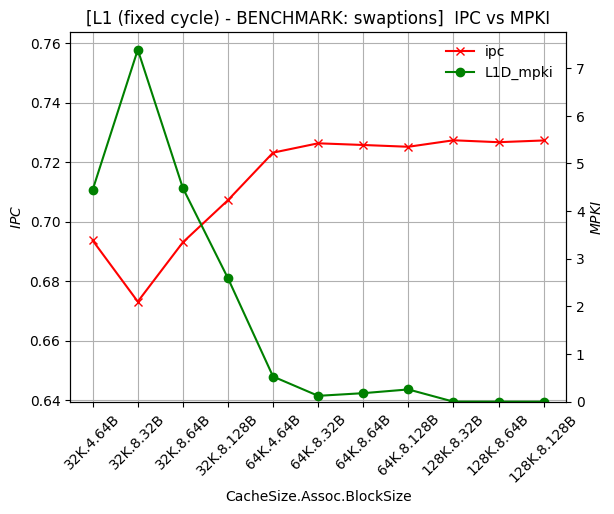
\includegraphics[scale=0.65]{graphs/L1/fixed/swaptions.png}
        \vspace{6mm}
    \end{center}
\end{minipage}

Επίσης, για λόγους συνολικής εποπτείας παρατίθεται ένα διάγραμμα των γεωμετρικών μέσων των προηγούμενων:\\\\
\begin{minipage}{\textwidth}
    \begin{center}
        \fbox{\textlatin{\textbf{\textit{Geometric Average}}}}\\
        \vspace{3mm}
        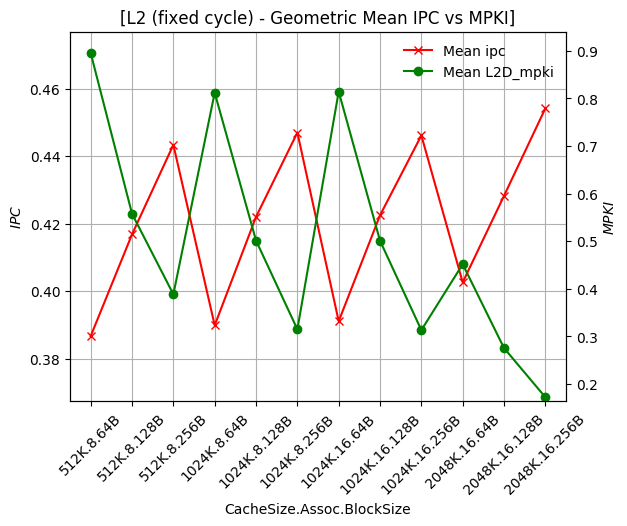
\includegraphics[scale=0.60]{graphs/L2/fixed/mean.png}
        \vspace{6mm}
    \end{center}
\end{minipage}

\begin{center}
    \textbf{Συμπεράσματα για την \textlatin{L2 Cache}}    
\end{center}

Και σε αυτή την περίπτωση παρατηρούμε πως τα μεγέθη Instructions Per Cycle και
Misses Per KiloInstructions μεταβάλλονται αντιστρόφως ανάλογα. Αυτό σαφώς είναι
αναμενόμενο, αφού όσο περισσότερες αστοχίες υπάρχουν (μεγαλύτερο MPKI), τόσο
περισσότεροι κύκλοι χρειάζονται για να εκτελεστεί η εντολή και άρα η επίδοση θα
είναι χειρότερη, δηλαδή το IPC θα είναι μικρότερο, και αντίστροφα. 

\begin{enumerate}
    \item Στα \textlatin{benchmarks canneal, ferret, fluidanimate} παρατηρούμε
    ότι η αύξηση του μεγέθους της \textlatin{cache} προκαλεί τη βελτίωση της
    επίδοσης, οπότε και μειώνονται τα \textlatin{capacity misses}.  
    
    \item Στο \textlatin{benchmark blackscholes}, παρατηρούμε πως η επιλογή L2
    Cache Size 2048K επιφέρει δραστική βελτίωση της επίδοσης. Μάλιστα για
    την επιλογή αυτή, τα υπόλοιπα χαρακτηριστικά φαίνεται πως δεν επηρεάζουν
    πλέον την απόδοση περεταίρω.

    \item Ta \textlatin{benchmark blackscholes} και ferret επηρεάζονται
    περισσότερο από το \textlatin{associativity} η οποία λογικά οφείλεται σε
    μείωση των \textlatin{conflict misses}. Σε γενικές γραμμές, η αύξηση του
    \textlatin{associativity} δεν επηρεάζει αρνητικά.
    
    \item Στα \textlatin{benchmarks blackscholes, bodytrack, facesim, ferret,
    fluidanimate, rtview, streamcluster} είναι εμφανές ότι η αύξηση του
    \textlatin{block size} προκαλεί και αύξηση στο \textlatin{IPC}, ενώ τα
    \textlatin{compulsory misses} μειώνονται. 
    
    \item Το \textlatin{benchmark swaptions} δείχνει να επηρεάζεται λιγότερο από
    τις αλλαγές των παραμέτρων και διατηρεί σχεδόν σταθερό \textlatin{IPC}. Αυτό
    ίσως οφείλεται στο μέγεθος των δεδομένων που επεξεργάζεται και είτε
    χρησιμοποιεί συνεχώς τα ίδια \textlatin{blocks}, είτε όποια
    \textlatin{blocks} διώχνονται δεν απαιτούνται ξανά.

\end{enumerate}

Σε γενικές γραμμές λοιπόν, βλέπουμε και πάλι ότι τη μεγαλύτερη επίδραση στην
απόδοση έχει η μεταβολή του \textlatin{block size}, χωρίς να είναι
αμελητέες οι αλλαγές που προκύπτουν από την αύξηση-μείωση των \textlatin{cache
size} και \textlatin{associativity}.
\vspace{1cm}

\textit{Θα μπορούσαμε λοιπόν με τις παραπάνω μετρήσεις να πούμε πως οι συνδυασμοί
2048Κ.16.256Β και 2048Κ.16.256Β αποτελούν αρκετά καλές επιλογές για την \textlatin{L2 Cache}.}

\newpage


%----------------TLB-----------------------
\subsubsection{TLB}
Οι παράμετροι της \textlatin{L1 cache} και της \textlatin{L2 cache} θα
διατηρηθούν σταθερές και συγκεκριμένα ίσες με:

\begin{multicols}{2}
    \begin{itemize}
        \item L1 size = 32 KB  
        \item L1 associativity = 8
        \item L1 block size = 64 B
        \item L2 size = 1024 KB  
        \item L2 associativity = 8
        \item L2 block size = 128 B
    \end{itemize}
\end{multicols}


\vspace{2cm}
\begin{minipage}{\textwidth}
    \begin{center}
        \fbox{\textlatin{\textbf{\textit{blackscholes}}}}\\
        \vspace{3mm}
        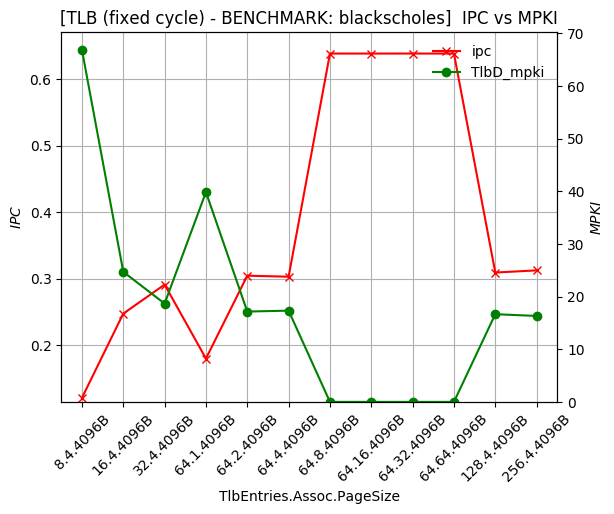
\includegraphics[scale=0.70]{graphs/TLB/fixed/blackscholes.png}
        \vspace{6mm}
    \end{center}
\end{minipage}


\begin{minipage}{\textwidth}
    \begin{center}
        \fbox{\textlatin{\textbf{\textit{bodytrack}}}}\\
        \vspace{3mm}
        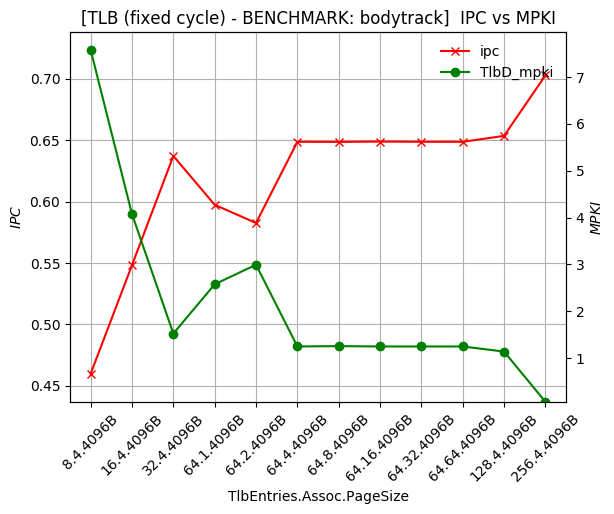
\includegraphics[scale=0.70]{graphs/TLB/fixed/bodytrack.png}
        \vspace{6mm}
    \end{center}
\end{minipage}

\begin{minipage}{\textwidth}
    \begin{center}
        \fbox{\textlatin{\textbf{\textit{canneal}}}}\\
        \vspace{3mm}
        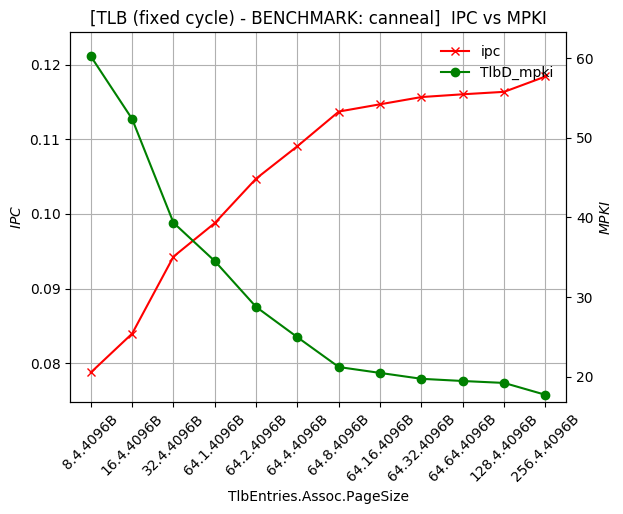
\includegraphics[scale=0.70]{graphs/TLB/fixed/canneal.png}
        \vspace{6mm}
    \end{center}
\end{minipage}

\begin{minipage}{\textwidth}
    \begin{center}
        \fbox{\textlatin{\textbf{\textit{facesim}}}}\\
        \vspace{3mm}
        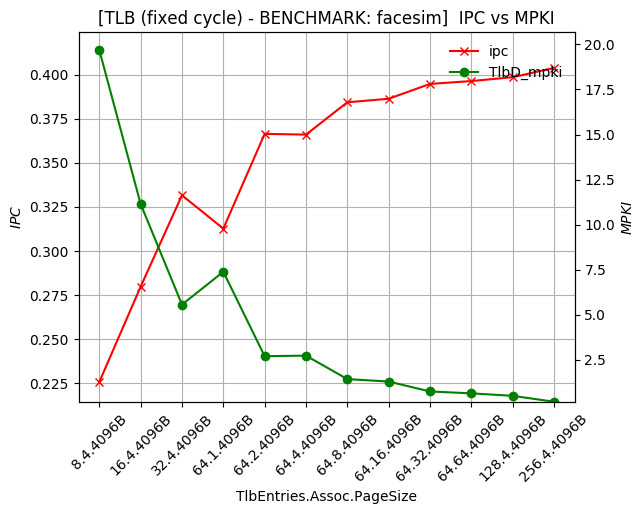
\includegraphics[scale=0.70]{graphs/TLB/fixed/facesim.png}
        \vspace{6mm}
    \end{center}
\end{minipage}

\begin{minipage}{\textwidth}
    \begin{center}
        \fbox{\textlatin{\textbf{\textit{ferret}}}}\\
        \vspace{3mm}
        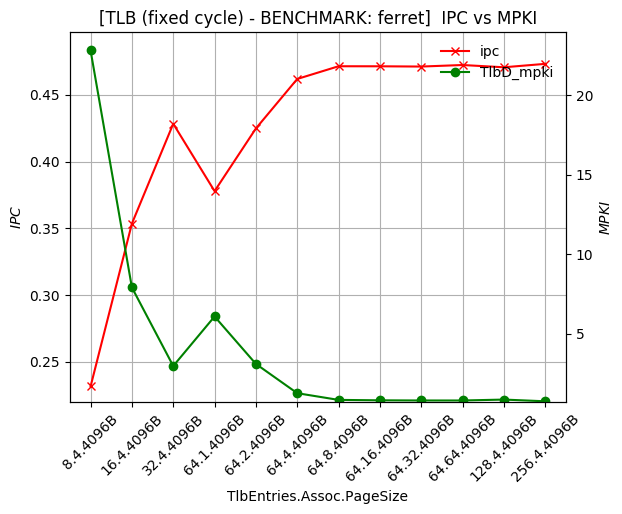
\includegraphics[scale=0.70]{graphs/TLB/fixed/ferret.png}
        \vspace{6mm}
    \end{center}
\end{minipage}


\begin{minipage}{\textwidth}
    \begin{center}
        \fbox{\textlatin{\textbf{\textit{fluidanimate}}}}\\
        \vspace{3mm}
        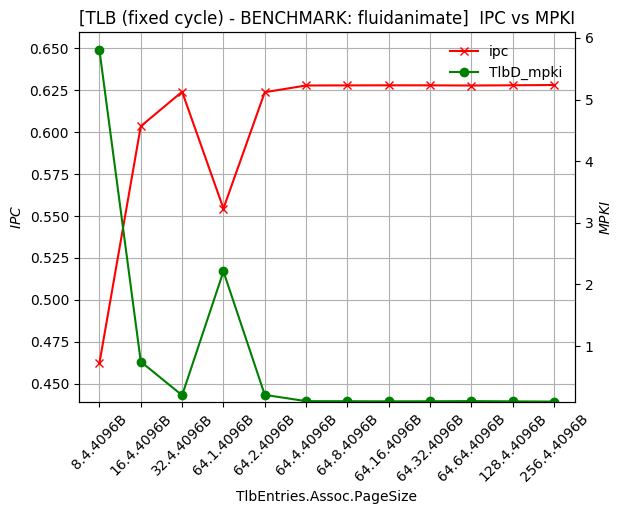
\includegraphics[scale=0.70]{graphs/TLB/fixed/fluidanimate.png}
        \vspace{6mm}
    \end{center}
\end{minipage}

\begin{minipage}{\textwidth}
    \begin{center}
        \fbox{\textlatin{\textbf{\textit{freqmine}}}}\\
        \vspace{3mm}
        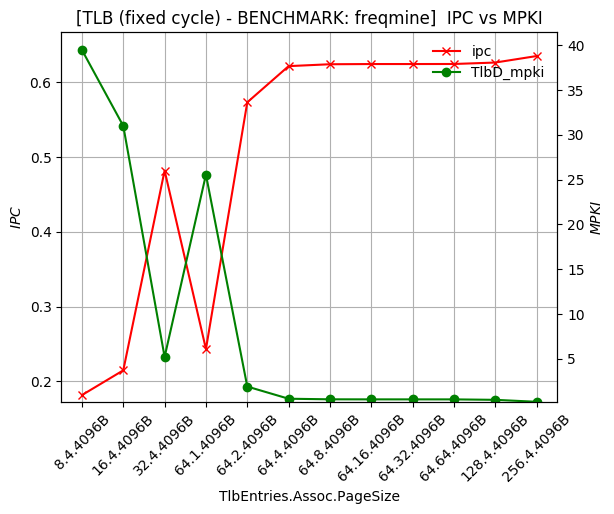
\includegraphics[scale=0.70]{graphs/TLB/fixed/freqmine.png}
        \vspace{6mm}
    \end{center}
\end{minipage}

\begin{minipage}{\textwidth}
    \begin{center}
        \fbox{\textlatin{\textbf{\textit{rtview}}}}\\
        \vspace{3mm}
        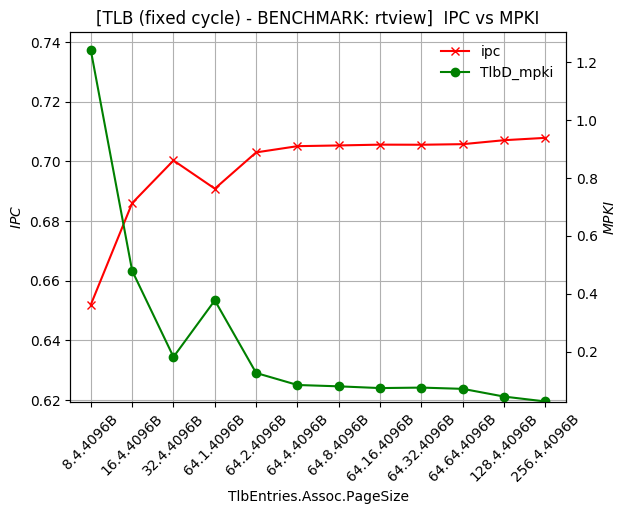
\includegraphics[scale=0.70]{graphs/TLB/fixed/rtview.png}
        \vspace{6mm}
    \end{center}
\end{minipage}

\begin{minipage}{\textwidth}
    \begin{center}
        \fbox{\textlatin{\textbf{\textit{streamcluster}}}}\\
        \vspace{3mm}
        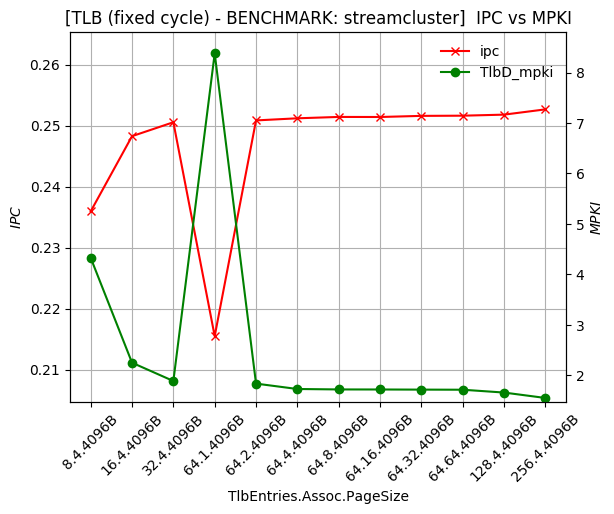
\includegraphics[scale=0.70]{graphs/TLB/fixed/streamcluster.png}
        \vspace{6mm}
    \end{center}
\end{minipage}

\begin{minipage}{\textwidth}
    \begin{center}
        \fbox{\textlatin{\textbf{\textit{swaptions}}}}\\
        \vspace{3mm}
        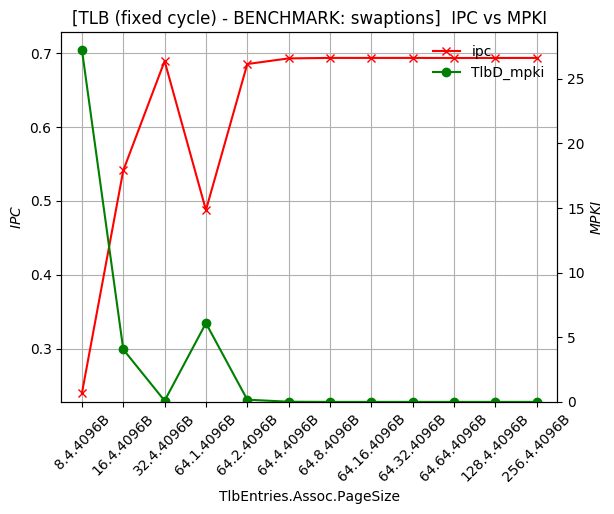
\includegraphics[scale=0.70]{graphs/TLB/fixed/swaptions.png}
        \vspace{6mm}
    \end{center}
\end{minipage}

Επίσης, για λόγους συνολικής εποπτείας παρατίθεται ένα διάγραμμα των γεωμετρικών μέσων των προηγούμενων:\\\\
\begin{minipage}{\textwidth}
    \begin{center}
        \fbox{\textlatin{\textbf{\textit{Geometric Average}}}}\\
        \vspace{3mm}
        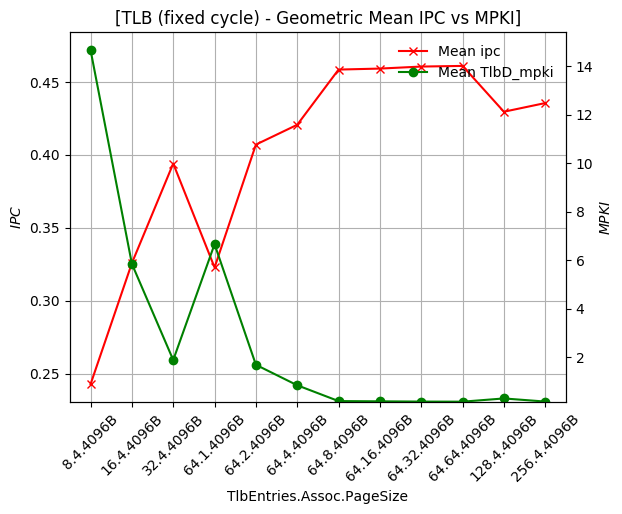
\includegraphics[scale=0.60]{graphs/TLB/fixed/mean.png}
        \vspace{6mm}
    \end{center}
\end{minipage}

\begin{center}
    \textbf{Συμπεράσματα για το \textlatin{TLB}}    
\end{center}

Αναμενόμενα παρατηρούμε να μεταβάλλονται αντιστρόφως ανάλογα τα μεγέθη
\textlatin{IPC, MPKI}. Αυτό είναι λογικό αφού όσο περισσότερες αστοχίες
γίνονται, τόσο χειρότερη επίδοση θα έχουμε (άρα μικρότερο \textlatin{IPC})
και αντίστροφα. 

\begin{enumerate}
    \item Σε όλα τα \textlatin{benchmarks}, παρατηρούμε ότι η αύξηση του
    \textlatin{TLB size} έχει ως αποτέλεσμα την αύξηση του \textlatin{IPC},
    οπότε και τη μείωση των \textlatin{misses}. Ώστόσο, σε όλα τα
    μετροπρογράμματα με εξαίρεση ίσως των \textlatin{blackscholes,
    bodytrack}, η συνεχής αύξηση του \textlatin{TLB size} πάνω από 64Β ή 128Β
    δεν προσέφερε κάποια ουσιαστική αλλαγή στην απόδοση.
    
    \item Όσον αφορά το \textlatin{associativity}, παρατηρούμε σε όλα τα
    \textlatin{benchmarks} ότι συμβάλει θετικά στην αύξηση της απόδοσης, ωστόσο
    μέχρι ένα όριο. Στα περισσότερα, η απόδοση είχε σημαντική βελτίωση μέχρι το
    \textlatin{associativity} να πάρει τιμές από 4 έως 8, αλλά απο εκεί και
    πάνω, δεν υπήρχε κάποια αξιοσημείωτη μεταβολή.
    
    \item Για το \textlatin{TLB page} δεν μπορούμε να εξάγουμε κάποιο
    συμπέρασμα, δίοτι μας δίνεται σε όλες τις μετρήσεις ίσο με 4096Β.
    
    \item Δεν υπήρχε κάποιο \textlatin{benchmark} του οποίου δεν επηρεάστηκε η
    απόδοση και οι αστοχίες μετά τη μεταβολή των παραμέτρων.
\end{enumerate}


Γενικά λοιπόν, λαμβάνοντας υπόψιν και το διάγραμμα των γεωμετρικών μέσων τιμών,
διαπιστώνουμε ότι τόσο το μέγεθος του \textlatin{TLB}, όσο και η
το associativity παίζουν σημαντικό ρόλο στην επίδοση, μέχρι ενός ορίου.
Από ένα σημείο και πέρα η αύξησή τους δεν επηρεάζει σημαντικά, ούτε στο
\textlatin{IPC}, ούτε στα \textlatin{misses}.
\vspace{1cm}

\textit{Μπορούμε με τις παραπάνω μετρήσεις και διαγράμματα για το
\textlatin{TLB}, να διαλέγουμε ως αρκετά καλή επιλογή χαρακτηριστών το συνδυασμό
64.8.4096Β.}



\newpage
%----------------PREF-----------------------
\subsubsection{Prefetching}
Οι παράμετροι της \textlatin{L1 cache} και της \textlatin{L2 cache} και
\textlatin{TLB} θα διατηρηθούν σταθερές και συγκεκριμένα ίσες με:

\begin{multicols}{2}
    \begin{itemize}
        \item L1 size = 32 KB  
        \item L1 block size = 64 B
        \item L1 associativity = 8
        \item L2 size = 1024 KB  
        \item L2 block size = 128 B
        \item L2 associativity = 8
        \item TLB size = 64 entries  
        \item TLB associativity = 4
        \item TLB page size = 4096 B
    \end{itemize}
\end{multicols}


\vspace{1cm}
\begin{minipage}{\textwidth}
    \begin{center}
        \fbox{\textlatin{\textbf{\textit{blackscholes}}}}\\
        \vspace{3mm}
        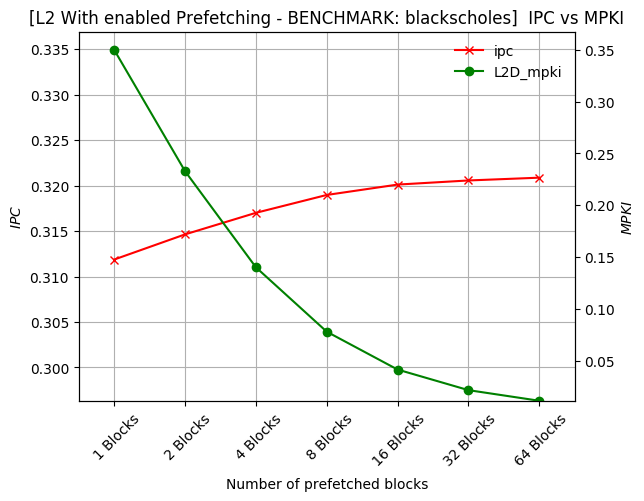
\includegraphics[scale=0.70]{graphs/PREF/blackscholes.png}
        \vspace{6mm}
    \end{center}
\end{minipage}


\begin{minipage}{\textwidth}
    \begin{center}
        \fbox{\textlatin{\textbf{\textit{bodytrack}}}}\\
        \vspace{3mm}
        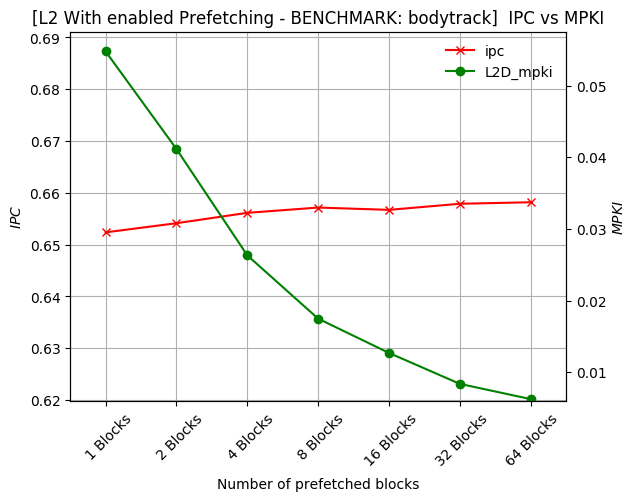
\includegraphics[scale=0.70]{graphs/PREF/bodytrack.png}
        \vspace{6mm}
    \end{center}
\end{minipage}

\begin{minipage}{\textwidth}
    \begin{center}
        \fbox{\textlatin{\textbf{\textit{canneal}}}}\\
        \vspace{3mm}
        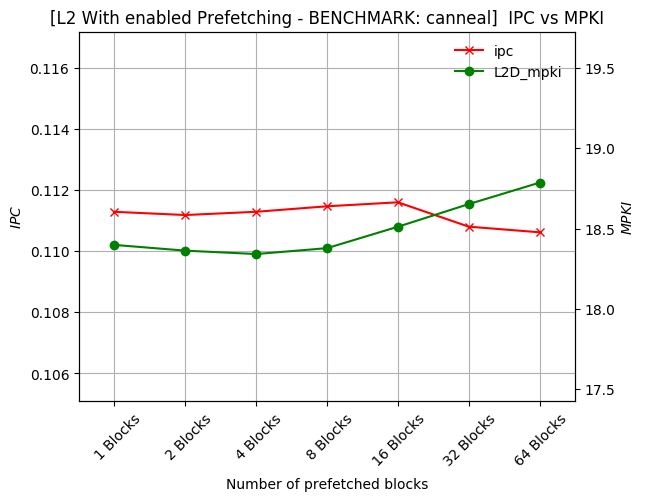
\includegraphics[scale=0.70]{graphs/PREF/canneal.png}
        \vspace{6mm}
    \end{center}
\end{minipage}

\begin{minipage}{\textwidth}
    \begin{center}
        \fbox{\textlatin{\textbf{\textit{facesim}}}}\\
        \vspace{3mm}
        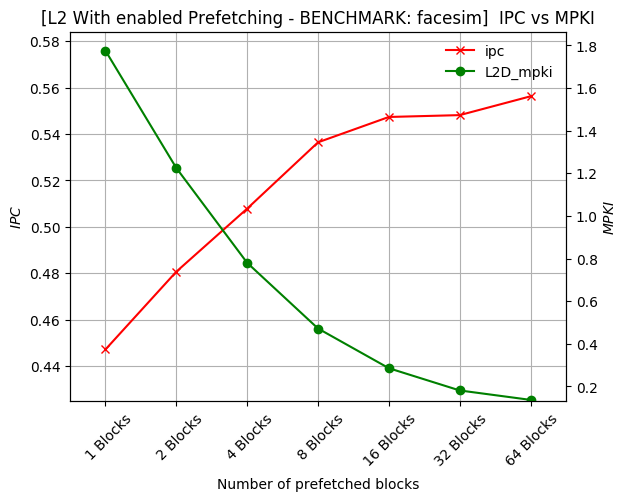
\includegraphics[scale=0.70]{graphs/PREF/facesim.png}
        \vspace{6mm}
    \end{center}
\end{minipage}

\begin{minipage}{\textwidth}
    \begin{center}
        \fbox{\textlatin{\textbf{\textit{ferret}}}}\\
        \vspace{3mm}
        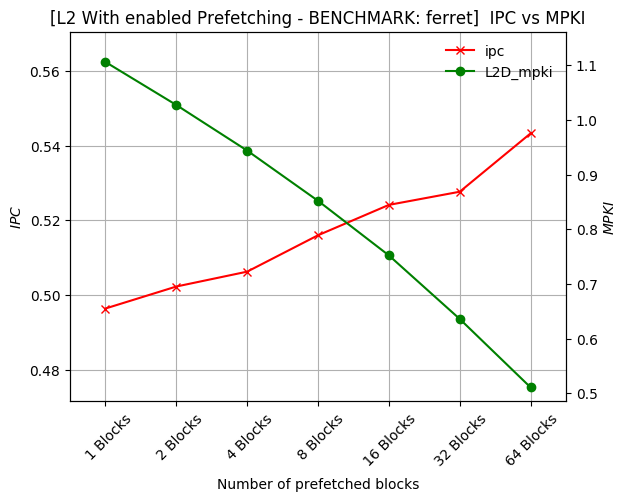
\includegraphics[scale=0.70]{graphs/PREF/ferret.png}
        \vspace{6mm}
    \end{center}
\end{minipage}


\begin{minipage}{\textwidth}
    \begin{center}
        \fbox{\textlatin{\textbf{\textit{fluidanimate}}}}\\
        \vspace{3mm}
        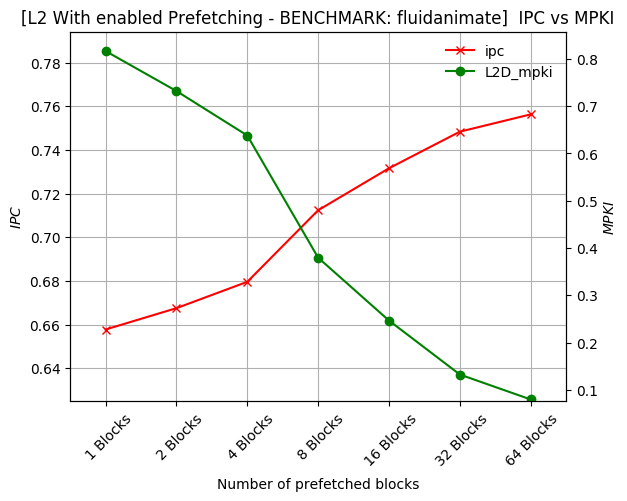
\includegraphics[scale=0.70]{graphs/PREF/fluidanimate.png}
        \vspace{6mm}
    \end{center}
\end{minipage}

\begin{minipage}{\textwidth}
    \begin{center}
        \fbox{\textlatin{\textbf{\textit{freqmine}}}}\\
        \vspace{3mm}
        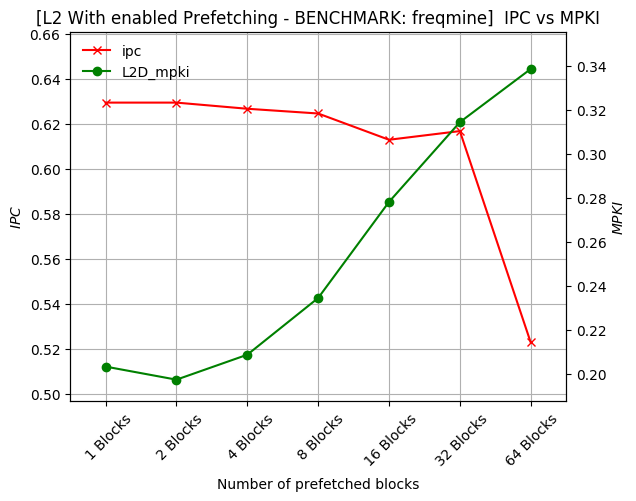
\includegraphics[scale=0.70]{graphs/PREF/freqmine.png}
        \vspace{6mm}
    \end{center}
\end{minipage}

\begin{minipage}{\textwidth}
    \begin{center}
        \fbox{\textlatin{\textbf{\textit{rtview}}}}\\
        \vspace{3mm}
        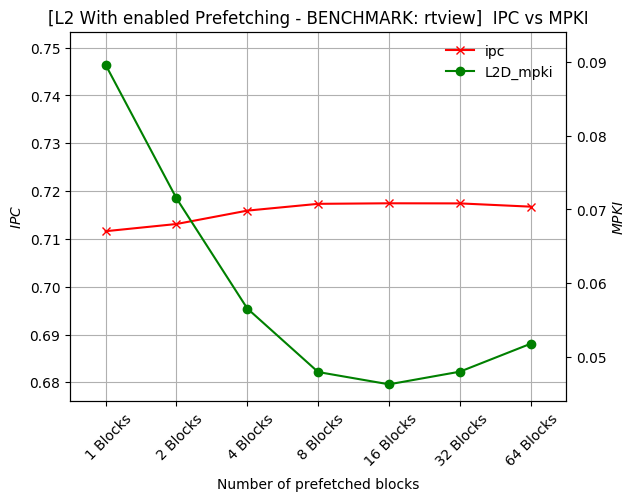
\includegraphics[scale=0.70]{graphs/PREF/rtview.png}
        \vspace{6mm}
    \end{center}
\end{minipage}

\begin{minipage}{\textwidth}
    \begin{center}
        \fbox{\textlatin{\textbf{\textit{streamcluster}}}}\\
        \vspace{3mm}
        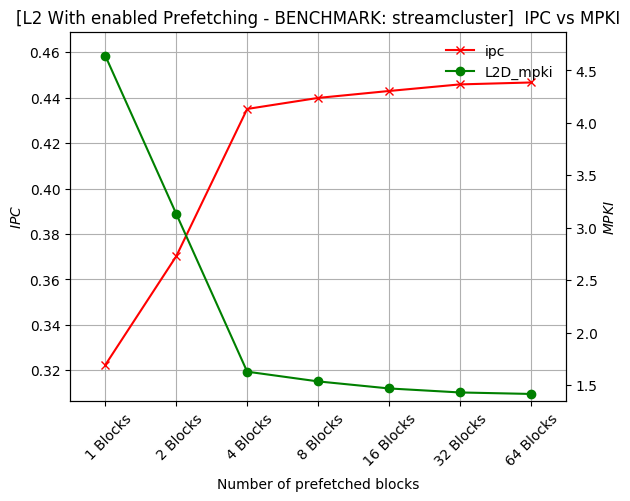
\includegraphics[scale=0.70]{graphs/PREF/streamcluster.png}
        \vspace{6mm}
    \end{center}
\end{minipage}

\begin{minipage}{\textwidth}
    \begin{center}
        \fbox{\textlatin{\textbf{\textit{swaptions}}}}\\
        \vspace{3mm}
        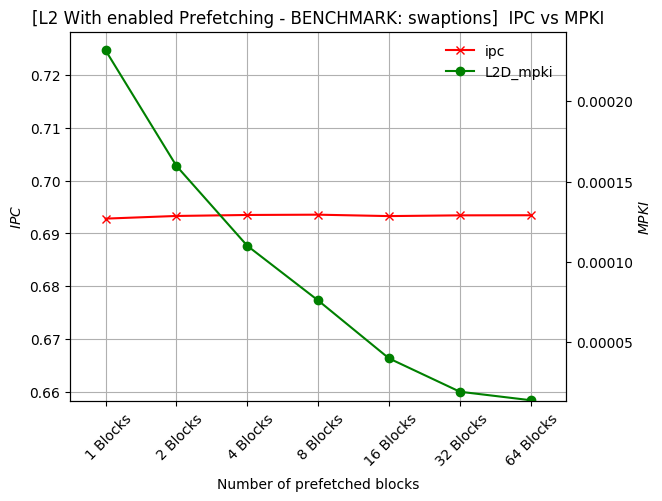
\includegraphics[scale=0.70]{graphs/PREF/swaptions.png}
        \vspace{6mm}
    \end{center}
\end{minipage}



\begin{minipage}{\textwidth}
    \begin{center}
\textbf{Συμπεράσματα για το \textlatin{Prefetching}}    
    \end{center}
\end{minipage}

\begin{enumerate}
    \item Παρατηρούμε πως υπάρχουν \textlatin{benchmarks}, στα οποία δεν
    επηρεάζεται σχεδόν καθόλου το \textlatin{IPC} τους από το
    \textlatin{prefetching}. Αυτά είναι τα εξής: \textlatin{blackscholes (IPC}
    στο διάστημα $0.31-0.32$ περίπου), \textlatin{bodytrack (IPC} στο διάστημα
    $0.65-0.66$ περίπου), \textlatin{canneal (IPC} στο διάστημα $0.110-0.112$
    περίπου), \textlatin{rtview (IPC} στο διάστημα $0.71-0.72$ περίπου),
    \textlatin{swaptions (IPC} στο διάστημα $0.690-0.695$ περίπου). Λόγω αυτής
    της συμπεριφοράς, μπορούμε να συμπεράνουμε πως οι προσπελάσεις δεν γίνονται
    σε διαδοχικά \textlatin{blocks}.
    
    \item Στα \textlatin{benchmarks facesim, ferret, fluidanimate,
    streamcluster}  παρατηρούμε ότι παρουσιάζουν σημαντική βελτίωση στο
    \textlatin{IPC} τους για αυξανόμενο πλήθος \textlatin{prefetched blocks}.
    
    \item Στο \textlatin{benchmark freqmine} βλέπουμε ότι παρουσιάζει κατά κύριο
    λόγο μείωση του \textlatin{IPC} με την αύξηση του πλήθους των
    \textlatin{prefetched blocks}. Αυτό μπορεί να συμβαίνει διότι κατά το
    \textlatin{prefetching}, κάποια \textlatin{block} στην \textlatin{cache}
    αντικαθίστανται υποχρεωτικά από άλλα, και αν φεύγουν συνεχώς αυτά που
    χρειάζεται το πρόγραμμα, θα αυξάνονται τα \textlatin{misses}.

\end{enumerate}

Σε γενικές γραμμές λοιπόν, βλέπουμε ότι το \textlatin{prefetching} είναι
επιθυμητό και επιδρά θετικά στην αύξηση της επίδοσης των προγραμμάτων μέχρι ενός ορίου.\vspace{1cm}